\documentclass[letterpaper, 12pt]{article}
\usepackage{graphicx}
\usepackage{amsmath}
\usepackage{wrapfig}
\usepackage{geometry}
\usepackage{float}
\geometry{margin= 1in}

  
\title{%
    Crane Project Report \\
\large ME 201
}

\author{Warner Vance, Sam Sierra, Malini Krejcarek}
\date{23 August 2024}

\begin{document}
\maketitle
\begin{figure}[H]
    \centering
    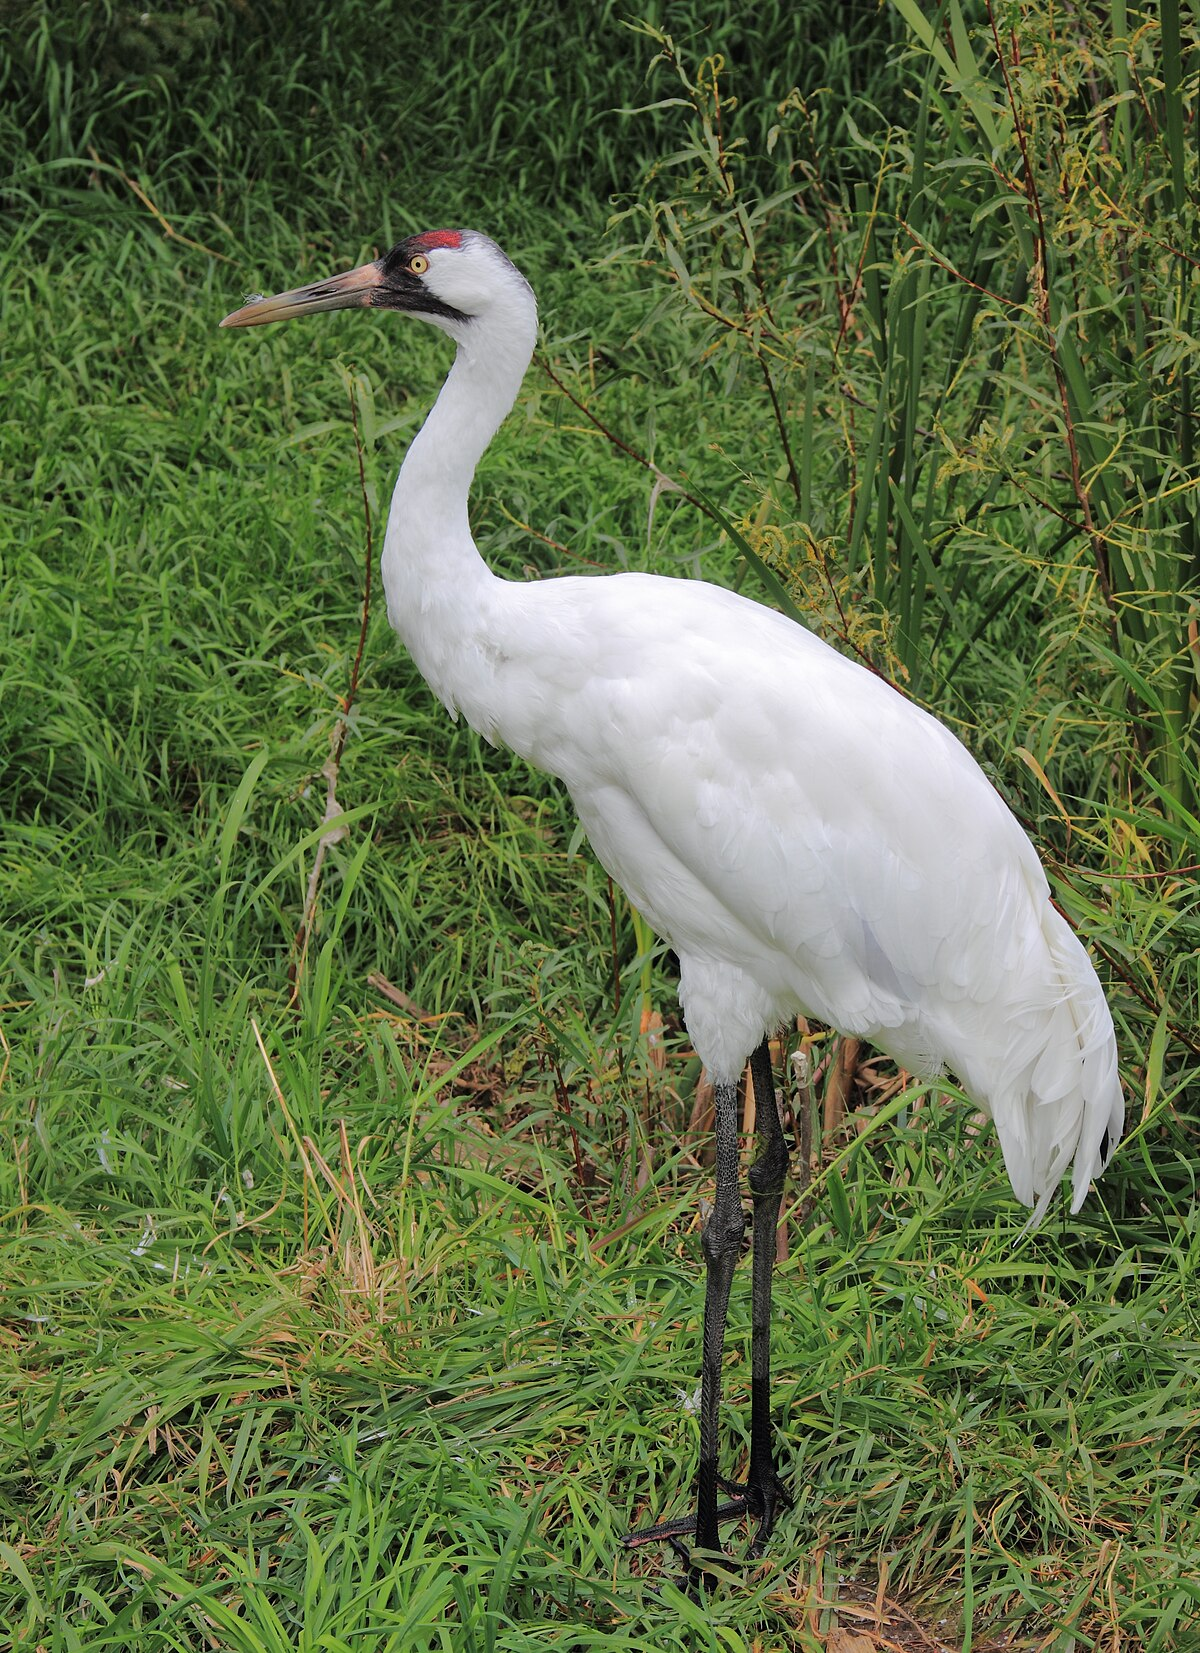
\includegraphics[scale = 0.1]{American Crane Sasata.jpg}
    \caption{A Crane}
\end{figure}
\begin{center}
    \LARGE What's a crane's favorite type of music?\\
    \Large Heavy Metal. \\
    \footnotesize Malini Krejcarek \\
    \tiny Noted Philosopher \\
\end{center}

    

\section{Introduction}
The goal of this project was to make a crane capable of lifting a heavy object as fast as possible using as little mass as possible. 
We were given a chassis, motors, pulleys,  and a micro-controller, everything else we had to make ourselves. 
This includes several aluminum scaffolding components, a base made of HDPE, structural braces, and a wooden support implement. 

\section{Design: Warner}

\subsection{Pulley System}
\label{sec:Pulley}
We decided early on make a simple crane, so that we could focus our efforts on optimization.
We wanted to lift 2.1 kg, and we designed the crane around it. 
We did some quick math and determined that a block and tackle system that split the tension in half would be best. 
Using a spreadsheet, we came up with an equation for the relationship between torque and rotational speed of a motor. 
This equation was then multiplied by two to account for the fact that two motors were being used. 
This equation was then put into EES along with an equation that related the torque to the radius of the pulley and the weight of the object being pulled up.

\begin{figure}[H]
    \centering
    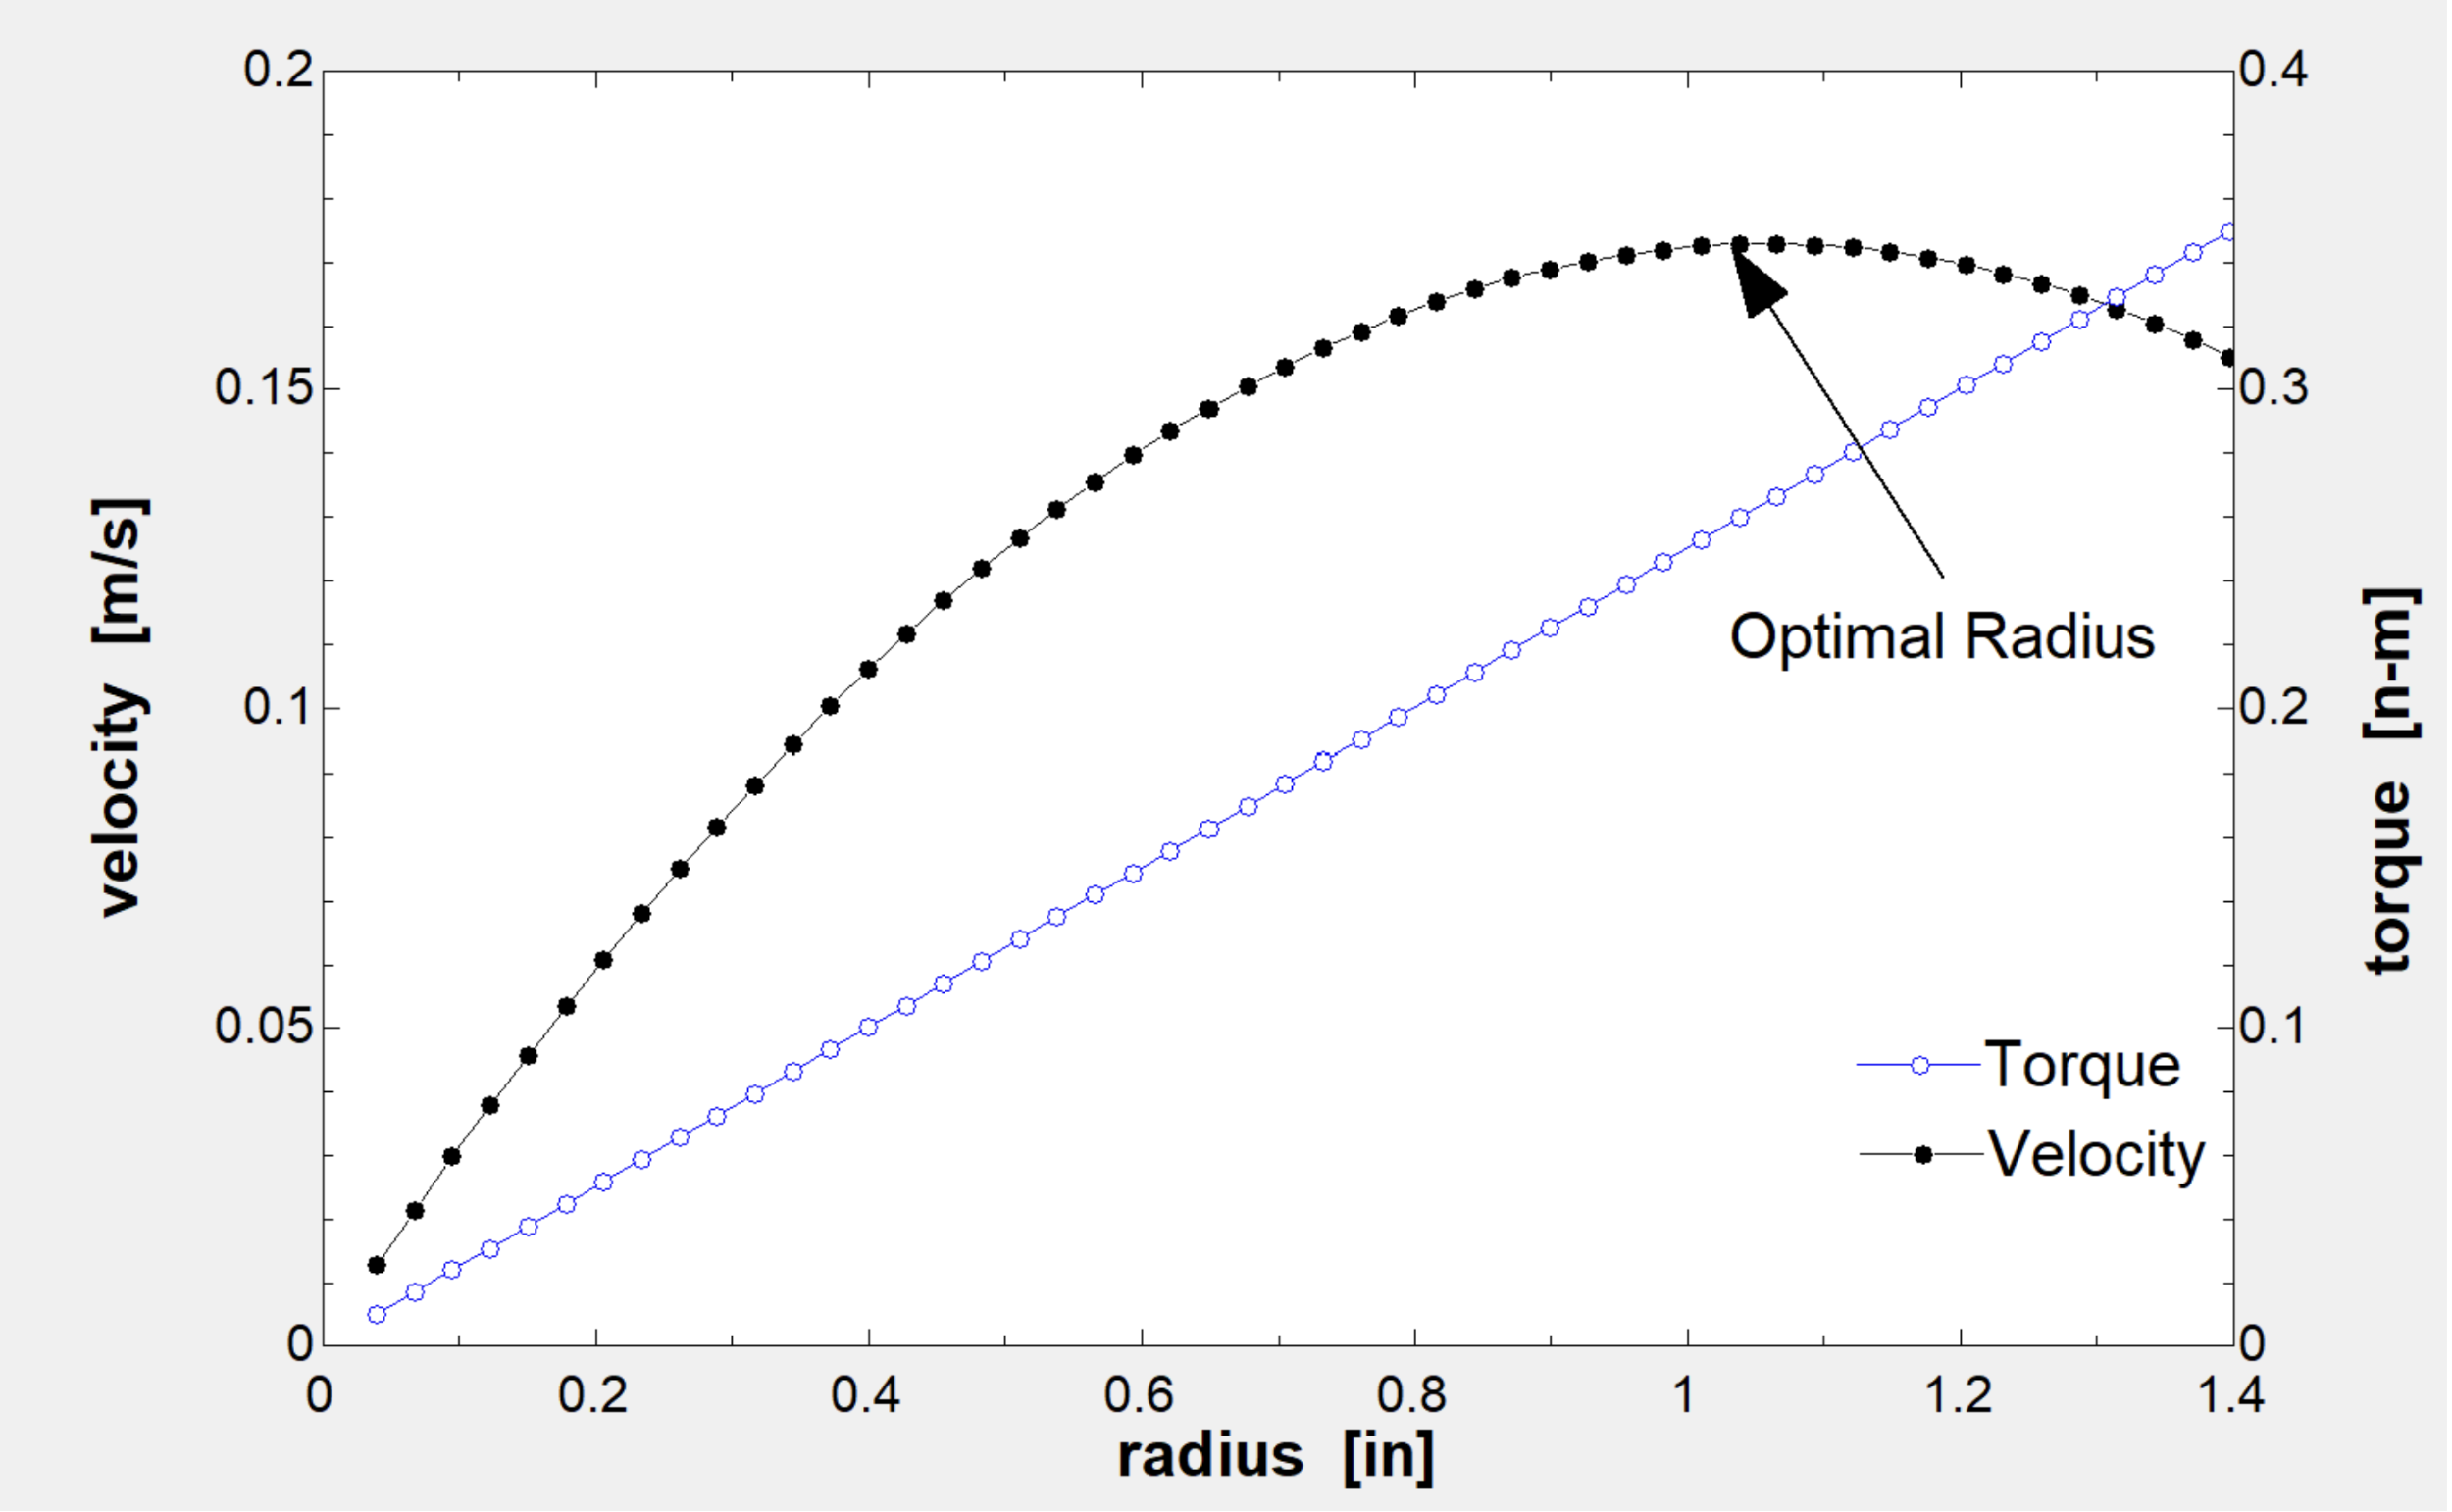
\includegraphics[width =.45\linewidth]{Torque_Speed.png}
    \caption{A graph of the relationship between the radius of the drive pulley and the vertical velocity of the object being lifted. Torque delivered from the motors is also included for reference.}
    \label{fig:Torque_Speed}
\end{figure}

We derived the vertical velocity of the object using equation \ref{eq:Velocity}.
\begin{equation}
    \begin{split}
        \text{Velocity}=\frac{2*\pi*{\text{Radius}*\text{Rotational Speed}}}{\text{Number of Lines connected to bucket}}     \label{eq:Velocity} //
        \text{torque}=-0.1294*\text{rotational speed}+0.2649 \\
    \end{split}
\end{equation}
Where:
\begin{equation}
    \begin{split}
       & \text{Velocity} \text{ is the vertical velocity of the object being lifted} \\
        &\text{Radius}  \text{ is the radius of the drive pulley} \\
        &\text{Rotational Speed}  \text{ is the rotational speed of the drive pulley} \\
        &\text{Number of Lines connected to bucket}  \text{ is the number of lines connected to the bucket}
    \end{split}
\end{equation}

The subsequent parametric study and graph showed that 1 inch was the idea drive pulley radius because it maximized the vertical velocity of the object being lifted.  This can be seen in Figure \ref{fig:Torque_Speed}.

\subsection{Counterweight}
\label{sec:Counterweight}
We then moved on to calculating both the mass and the position of the counter weight. 
First we repeated an earlier lab procedure to find the center of mass of the crane using equations \ref{eq: CM1} to \ref{eq: CM2}.
\begin{figure}[H]
    \centering
    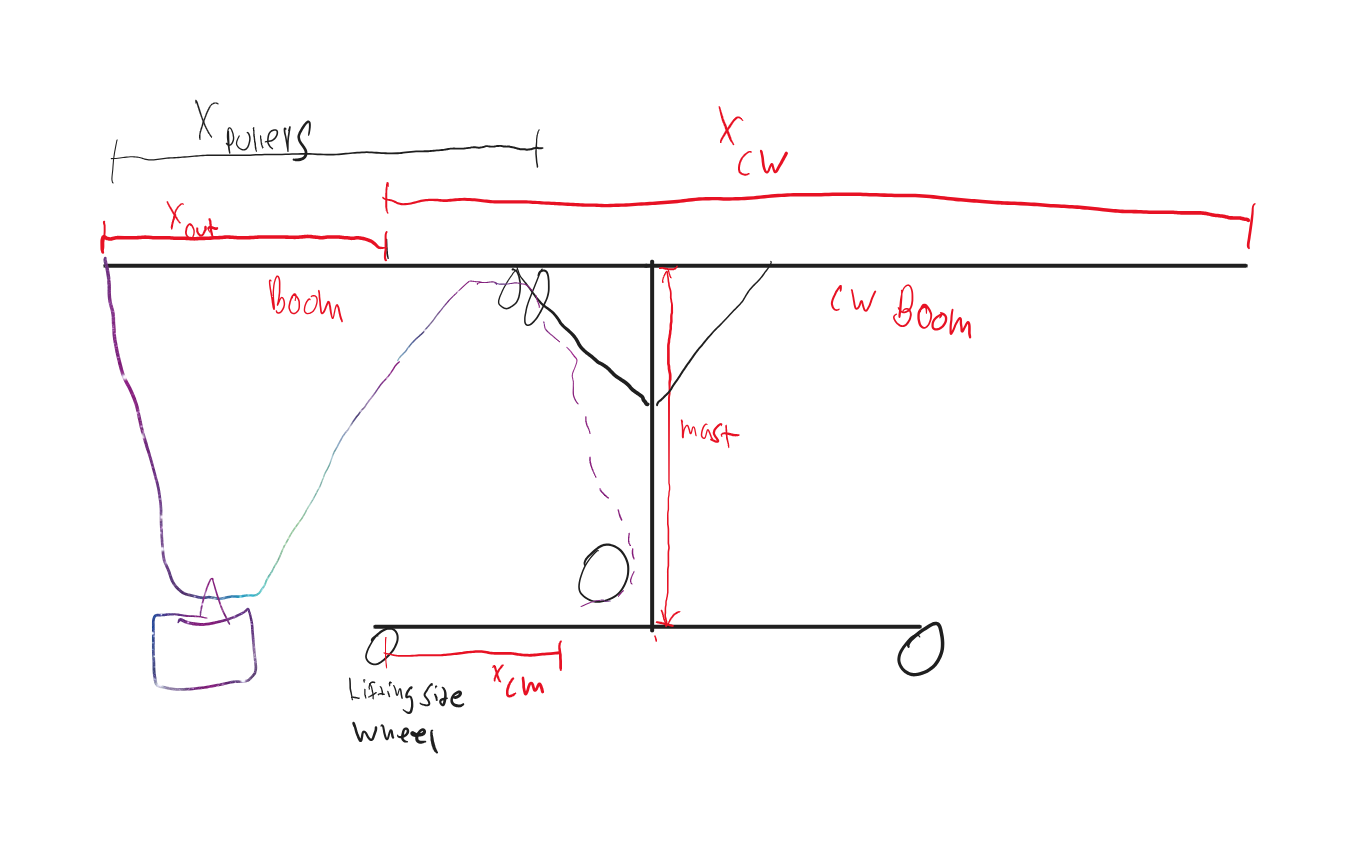
\includegraphics[width =0.6\linewidth]{null (3).png}
    \caption{A diagram of the crane}
    \label{fig:Crane}
\end{figure}

\begin{align}
        w_{\text{tip}}= & m_{\text{tip}} * 9.8 \label{eq: CM1} \\ 
        t_{\text{tip}}= & w_{\text{tip}}*x_{\text{out}}\label{eq:Torque 1} \\ 
        t_{\text{tip}}= & w_{\text{crane}}*x_{\text{cm}}\label{eq:Torque 2} \\
        x_{\text{cm}}= & \frac{t_{\text{tip}}}{w_{\text{crane}}} \label{eq: CM2}
\end{align}

\begin{equation}
    \begin{split}
        \text{Where:} \\
        m_{\text{tip}} & \text{ is the mass of the object that makes the crane tip} \\
        w_{\text{tip}} & \text{ is the weight of } m_{\text{tip}} \\
        x_{\text{out}} & \text{ is the x from the lifting side wheel to the where the mass is hung} \\
        t_{\text{tip}} & \text{ is the torque from the object that makes the crane tip} \\
        w_{\text{crane}} & \text{ is the weight of the crane without the counterweight} \\
        x_{\text{cm}} & \text{ is the x from the lifting side wheel to the center of mass of the crane.} \\
        \text{Note:} & \text{ Check figure \ref{fig:Crane} for a diagram of the crane.}
    \end{split}
\end{equation}



Equation \ref{eq:Torque 1} and \ref{eq:Torque 2} are made possible by the fact that at the moment of tipping the sum of the moments must be zero because nothing should be moving. 

Once the center of mass was found, we could then calculate the mass of the counterweight. A free body diagram of the pulleys can be found in figure \ref{fig:Pulleys}. This helps 
\begin{figure}
    \centering
    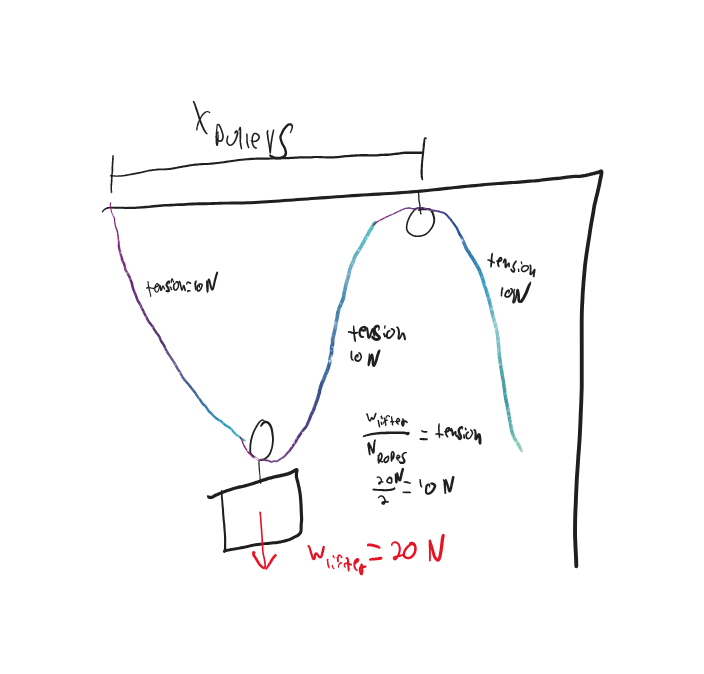
\includegraphics[width =0.6\linewidth]{null (2).png}
    \caption{A free body diagram of the pulleys}
    \label{fig:Pulleys}
\end{figure}

\begin{align}
& w_{\text{lift}}=m_{\text{lift}}*9.81 \\
& t_{\text{lift}}= \frac{w_\text{lift}}{2}*x_{\text{out}}+ w_{\text{lift}}*(x_\text{out}-x_{\text{pulleys}}) \footnotemark \label{eq:CW 1} \\ 
% (x_cm * w_crane) + (((x_wheels/2) + x_cw) * w_cw) = t_lift
& t_{\text{lift}} = x_{\text{cm}} * w_{\text{crane}} + x_{\text{cw}} * w_{\text{cw}} \label{eq: CW 2} \\
& m_{\text{cw}} = \frac{w_{\text{cw}}}{9.81}
\end{align}
\footnotetext{Equation \ref{eq:CW 1} was created when we only had one pulley attached to the boom. Luckily the calculated counterweight still worked when we added the second pulley.}
Where:
\begin{equation}
 \begin{split}
    & x_{\text{pulleys}}  \text{ is the distance betweens the pulleys and the anchor of the string on the boom } \\
    & x_{\text{cw}}  \text{ is the distance of the counterweight from the crane side wheel} \\
    & t_{\text{lift}} \text{ is the torque from the object being lifted} \\
    & m_{\text{lift}} \text{ is the mass of the object being lifted} \\
    & w_{\text{lift}} \text{ is the weight of the object being lifted} \\
 \end{split}
\end{equation}
Equations \ref{eq:CW 1} and \ref{eq: CW 2} are made possible by the fact that at the moment of lifting the sum of the moments must be zero because nothing should be moving.

This equation allowed us to perform a parametric study to find the ideal position and mass of the counterweight. The resulting graph can be seen in Figure \ref{fig:Counter Weight.png}.
\begin{figure}[H]
    \centering
    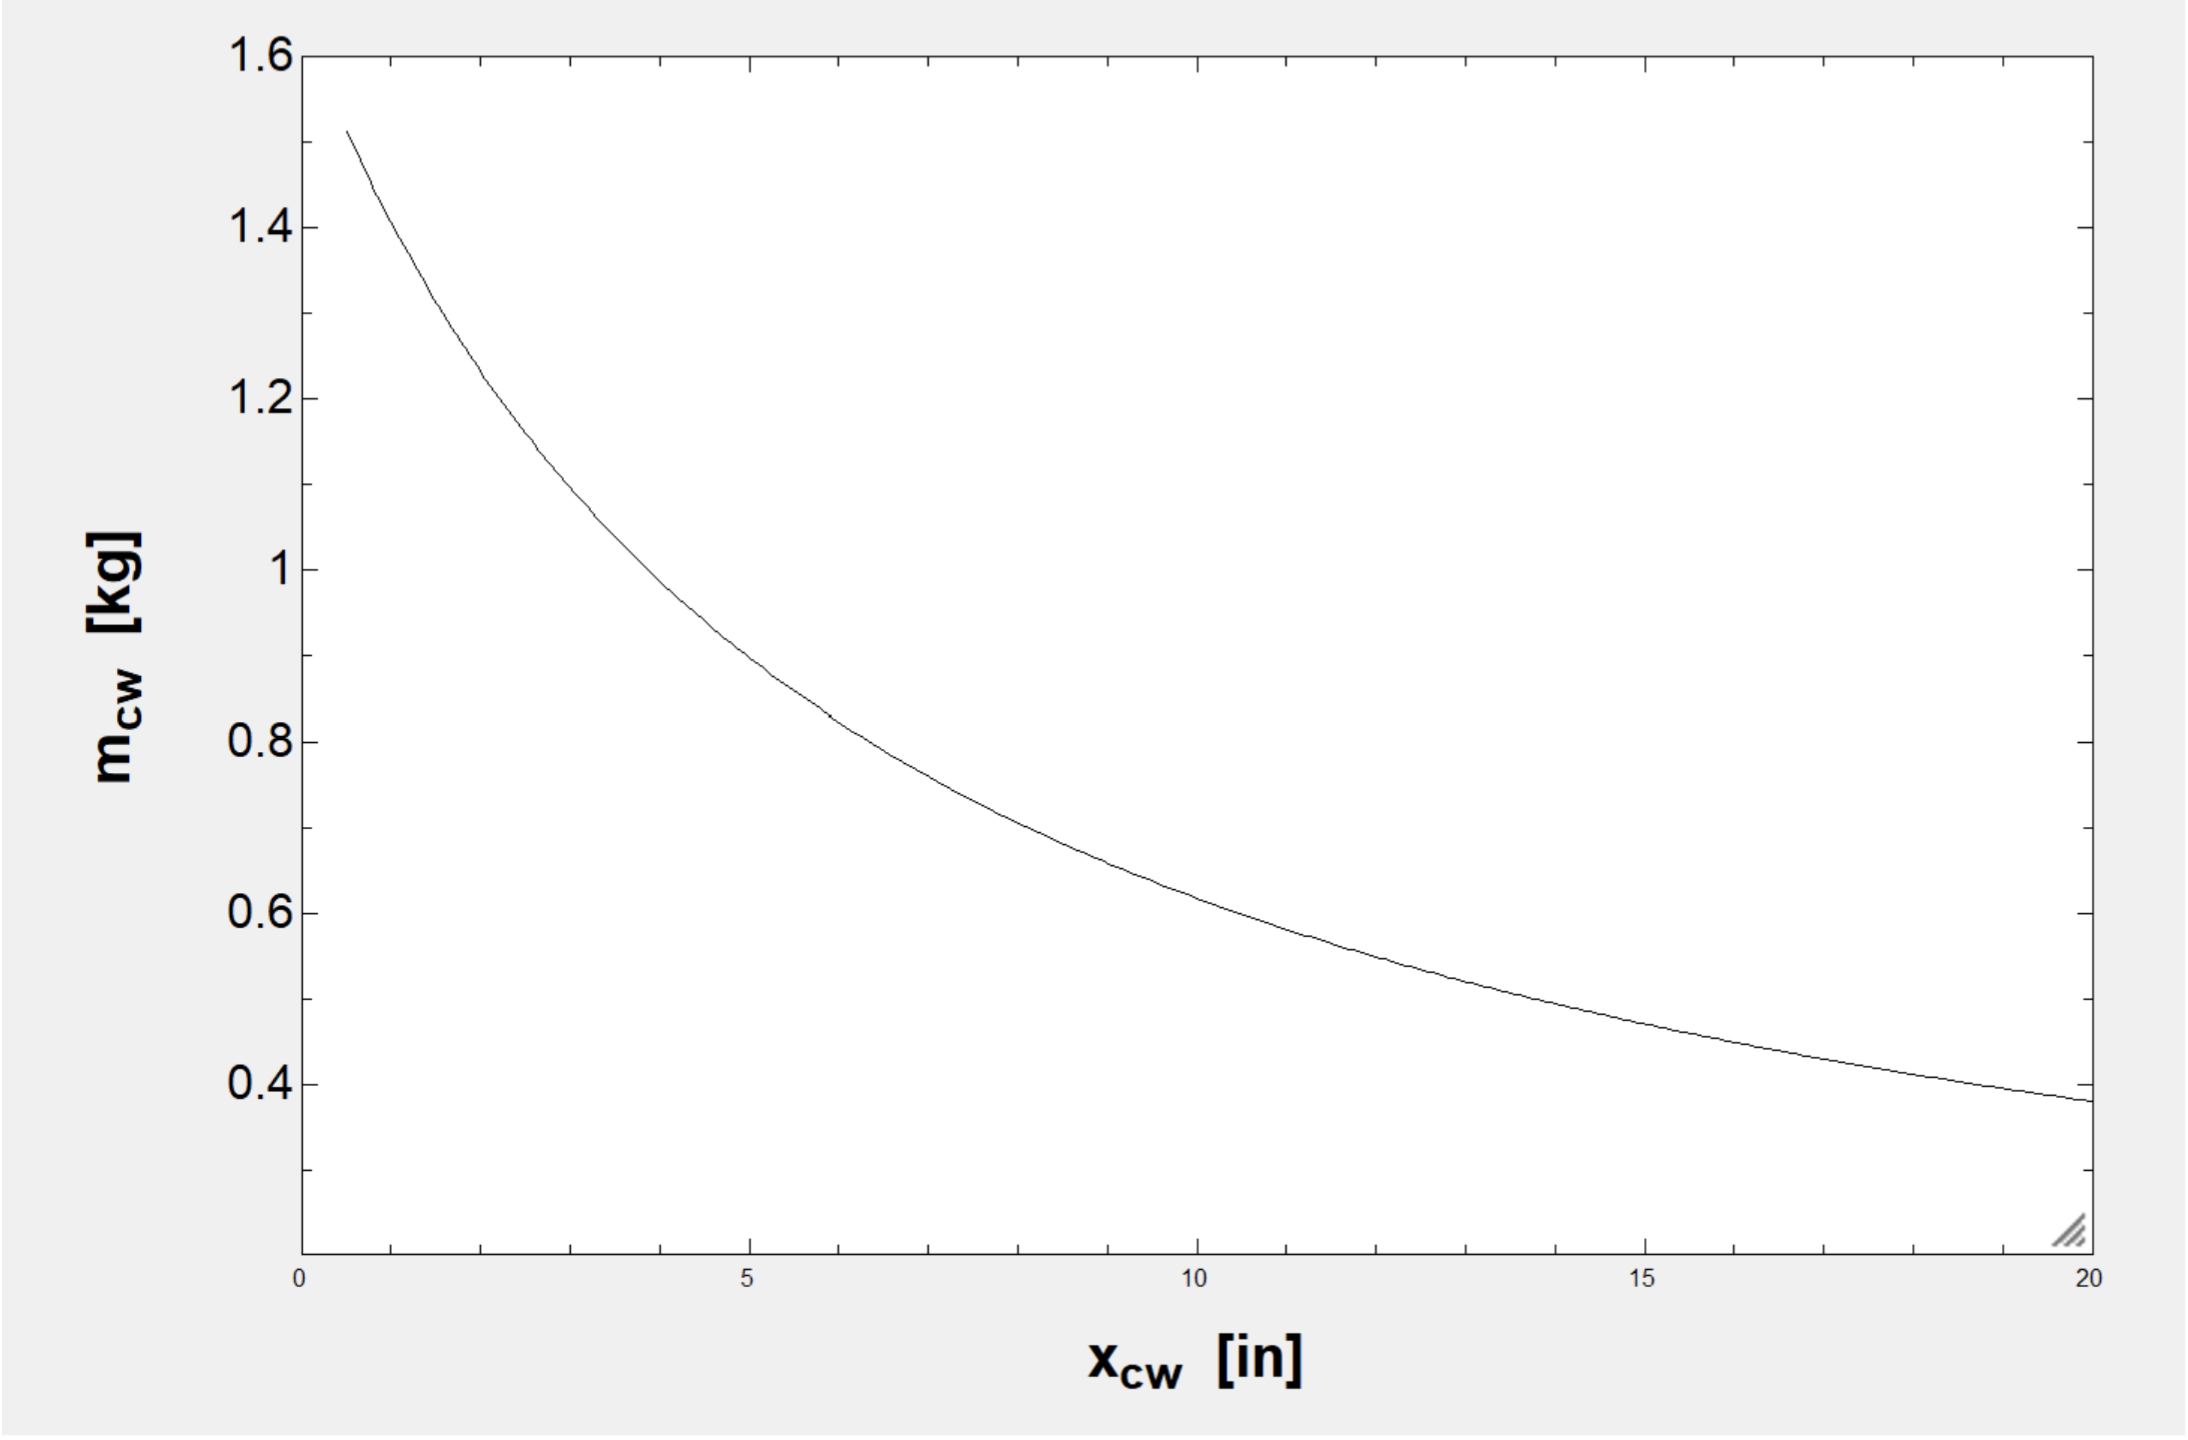
\includegraphics[width =.55\linewidth]{Counter Weight.png}
    \caption{A graph of the relationship between the mass of the counterweight and the vertical velocity of the object being lifted.}
    \label{fig:Counter Weight.png}
\end{figure}

Figure \ref{fig:Counter Weight.png} came in quite handy as we had to adjust the counterweight several times during the project.
Eventually we ended up making our counterweight boom 13 inches long\footnote{This distance refers to the distance from the center mast of to the end of the counterweight. This translates to a $x_{\text{cw}}$ of around 9.969 inches} which translated to a $m_{\text{cw}}$ of 0.7 kg.

\section{Construction: Sam }
\section{Testing: Malini}
\begin{figure}[H]
    \centering
    \includegraphics[width =.5\linewidth]{Screenshot 2024-08-22 at 3.47.12 PM.png}
    \caption{A picture of the crane before motor was attached.}
    \label{fig:pic of Crane}
\end{figure}

Before designing and building our crane, we tested many mechanisms of the crane through our labs in the ME 201 course. 
During the assessment, one of the key findings was the strength of the string, which is a crucial factor in determining the maximum weight our crane can lift. 
If the string breaks, it renders the crane ineffective.
Luckily, the assessment proved the string’s ability to support over 3 kilograms.
Once these preliminary tests were completed and project groups were assigned, tests went hand-in-hand with construction; we tested any new components as they were added, identifying any issues with said parts we designed and fabricated or simply obtained from the given resources in the lab. 
The first of such tests included merely our basic design for the lifting mechanism. 
This design included a crane mast and boom with our chosen pulley system attached (see Figure \ref{fig:pic of Crane}), and lacked any attachment to our three given motors. 
Manually, a team member raised the bucket through the pulley system to evaluate its stability and ensure fluidity of the movement and therefore a dependable base design to thenforth optimize. 

Next, my team initiated a test to determine if the first pulley we 3D printed from polylactic acid (PLA) in the Makerspace with the optimized radius of 1 inch (see figure \ref{fig:Torque_Speed}) for our system would have any issues in lifting the bucket. 
Having decided on a goal of at least 2.01 kilograms to be lifted by the crane, we tested the ability of the printed pulley to support this specific weight. 

When the pulley started to buckle, we reevaluated our use of PLA and that of a 3D printed part due to the hollow nature of the printing technique. 
Ultimately our team decided to reprint the part with more additional infill and layers of PLA for the walls. 
After bolstering the part yielded our replacement pulley, we swapped it for the previous pulley to stage a test otherwise identical to that prior. 
Although our ultimate design didn’t include this specific pulley due to issues attaching the material to th e motor, our findings in these two tests greatly benefitted our following design adaptations due to our greater understanding of the materials available in the Makerspace.


\section{Future Work}
The aspect of the crane designing/building process that we would likely do differently and our advice to future students have lots of overlap in that the advice of starting early should not be disregarded. 
While we started working right away, we were still overwhelmed by a great number of unknown variables in the equations and procedures that we needed to create and carry out. 
If we were to go back and reprise our approach to the project, our new attempt would involve us taking minimal time to assign values to variables that would be found subsequently (ex. mass of crane, length of counterweight deployment mechanism).

Pivoting to the question of what future projects we would like to see, there are many possibilities, as one of the leading attractions of the project was the great amount of creative freedom we had in designing our cranes. 
While also undoubtedly being the hardest part of the project, that liberty forced us to think through our choices more thoroughly than mere equations could. 
One idea that our team mentioned was a design inspired by crane arcade games to add another layer of excitement to the competition, and would require students to have some understanding of programming—which would be taught in the course—to control an opening and closing mechanism of the crane hand. 
Another idea was the use of centripetal force and a spinning crane to hit a target with some kind of attachment to the end of the string it lifts. 
This would also involve programming, as the crane must spin at a certain speed to stay on theme with work in the system, and calculations with respect to the position to which the crane must raise the string. 
Overall, we would love to see the creative nature of the project kept intact to continue to foster the growth in creativity, engineering application, and teamwork that our team experienced.




\end{document}